\documentclass[10pt]{article}

\usepackage{fancyhdr}
\usepackage[includeheadfoot,left=0.5in, right=0.5in, top=0.5in, bottom=0.5in]{geometry}
\usepackage{lastpage}
\usepackage{extramarks}
\usepackage[usenames,dvipsnames]{color}
\usepackage{graphicx}
\usepackage{listings}
\usepackage{courier}
\usepackage{float}
\usepackage{url}
\usepackage{subfigure}
\usepackage{varwidth}
\usepackage{caption}
\usepackage{multirow}
\usepackage[pdfborder={0 0 0}]{hyperref}
\usepackage[compact,small]{titlesec}
\usepackage{microtype}
\usepackage{verbatim}
\usepackage{booktabs}
\usepackage{indentfirst}
\usepackage{pgffor}

\parskip = 0.5\baselineskip
\setlength{\belowcaptionskip}{-\baselineskip}

\captionsetup{font=scriptsize}
\captionsetup{labelfont=bf}

\pagestyle{fancy}
\rhead{Max Thrun}
\lhead{EECS6083: Compiler Theory}
\rfoot{Page\ \thepage\ of \protect\pageref{LastPage}}
\cfoot{}
\renewcommand\headrulewidth{0.4pt}
\renewcommand\footrulewidth{0.4pt}

% make verbatim text small
%\makeatletter
%\g@addto@macro\@verbatim\tiny
%\makeatother

\setlength\parindent{0pt} % Removes all indentation from paragraphs

\title{
    \vspace{2in}
    \textmd{\textbf{EECS6083: Compiler Theory}}\\
    \vspace{4in}
}
\author{\textbf{Max Thrun}}

\begin{document}
\maketitle
\newpage
\section{Description}
This project implements a recursive decent parser-generator compiler for the
language specified in \texttt{projectLanguage.pdf}. The main compiler
source code is written in Python and can be found in the \texttt{src}
directory.  It is broken up into three major parts: token construction
(\texttt{src/scanner.py}), parsing (\texttt{src/parser.py}), and code
generation (\texttt{src/gen.py}).

Memory is provided via the runtime as an integer array. Storing floats is
accomplished by simply \texttt{memcpy}ing them into a slot in the memory array
which makes the assumption that both floats and integers are 4 bytes.  Strings
are defaulted to a max length of 100 characters and all strings allocate the
max length regardless of their actual size. Strings input by the user are
truncated at the 100 byte mark. All strings and arrays are passed via pointers
to and from procedures.

\section{Usage}

A wrapper script, \texttt{compiler.py}, is provided in the root directory of
the project which provides an easy way to both compile the test programs and
optionally run them after. Both the intermediate \texttt{.c} file and the final
executable have the same name and are placed in the same directory as the input
file. An example of compiling and running the \texttt{square\_array.src} test
file is shown below:

\begin{verbatim}
$ ./compiler.py -r tests/square_array.src
0 1 4 9 16 25 36 49 64 81
\end{verbatim}

The full usage of \texttt{compiler.py} is shown below.

\begin{verbatim}
usage: compiler.py [-h] [-c] [-r] filename

EECS 6083 Compiler

positional arguments:
  filename      input .src file

optional arguments:
  -h, --help    show this help message and exit
  -c, --c_only  only generate .c file, do not compile it
  -r, --run     run the program after compiling it
\end{verbatim}

\section{Error Messages}
A lot of time was spent trying to achieve the best possible error messages.
There are currently 57 unique error and warning messages. Message styling and
some phrasing were inspired by Clang. An example of some error messages from the
test file \texttt{tests/errors.src} are shown below.
\begin{figure}[H]
    \centering
    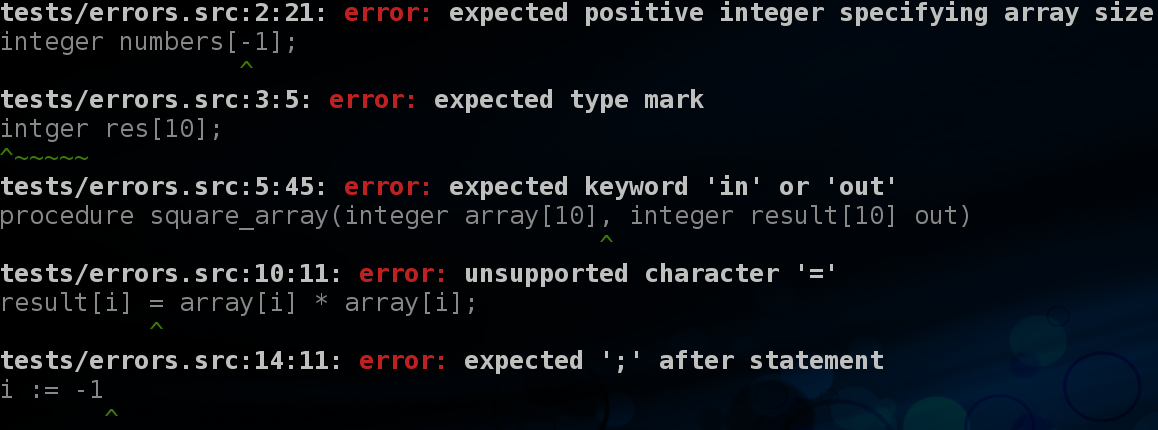
\includegraphics[width=0.75\linewidth]{./errors.png}
\end{figure}

\end{document}
